\input{../header}
\usepackage{parskip}
\usepackage{tabularx}
\everymath{\displaystyle}
\rhead{Your name: \rule{8cm}{0.15mm}}

\newcommand{\vtx}[2]{node[fill,circle,inner sep=0pt, minimum size=7pt,label=#1:#2]{}} 
\renewcommand{\v}{\vtx{above}{}} 

\begin{document}
%


%\onehalfspacing
\allowdisplaybreaks
%##################################################################
\section{Chapter 2 checkpoint!}

Scorecard!

\begin{center}
    \begin{tabular}{|m{3.75cm}|*{6}{m{1.75cm}|}} \hline
        Learning target: & P1 & P2 & L1 & L2 & L3 & L4 \\\hline
        Your confidence level before starting (0-5): & &&&&&\\\hline
        Your confidence level after the quiz (0-5): & &&&&&\\\hline
        The mark you earned on this attempt: 
        & Success! \newline Revise! \newline Try again!
        & Success! \newline Revise! \newline Try again!
        & Success! \newline Revise! \newline Try again!
        & Success! \newline Revise! \newline Try again!
        & Success! \newline Revise! \newline Try again!
        & Success! \newline Revise! \newline Try again! \\\hline
        &&&&&&\\\hline
        Learning target: & G1 & G2 & G3 & G4 &  & \\\hline
        Your confidence level before starting (0-5): & &&&&&\\\hline
        Your confidence level after the quiz (0-5): & &&&&&\\\hline
        The mark you earned on this attempt: 
        & Success! \newline Revise! \newline Try again!
        & Success! \newline Revise! \newline Try again!
        & Success! \newline Revise! \newline Try again!
        & Success! \newline Revise! \newline Try again! 
        & & \\\hline

    \end{tabular}
\end{center}

Before anything else, please do the following:
\begin{itemize}
    \item Rank your confidence from 0-5 on each of the learning targets. 5 means ``I could teach a whole class about this;'' 0 means ``I am genuinely not sure I have heard these words before.''
    \item Rip all the pages apart.
    \item Write your name on this page and on each of the other pages of the quiz.
\end{itemize}

Then do the quiz! Some reminders:
\begin{itemize}
    \item Open notes, closed computer.
    \item If you need more room to write, use the back of the same learning target page, or ask me for some scratch paper.
    \item Read the questions carefully and make sure you're answering each part.
    \item Show all your work and explain all your thinking!
\end{itemize}

When you are done:
\begin{itemize}
    \item Rank your confidence from 0-5 on each of the learning targets. 5 means ``I absolutely nailed that question for sure;'' 0 means ``oof, I definitely didn't get that one.''
    \item Make double sure your name is on every page, including any scratch paper.
    \item Hand in your work, separated by learning target.
\end{itemize}

Have fun and do your best! I believe in u $\heartsuit$

%%%%%%%%%%%%%%%%%%%%%%%%%%%%%%%%%%%%%%%%%%%%%%%%%%%%%%%%%
\pagebreak
%%%%%%%%%%%%%%%%%%%%%%%%%%%%%%%%%%%%%%%%%%%%%%%%%%%%%%%%%
\section{Learning target G1, version 1}

\begin{enumerate}
    \item Use the vertex set $V$ and edge set $E$ below to draw a picture of the graph $G = (V, E)$.
    \begin{align*}
        V = \{&a, b, c, d, e, f, g\} \\
        E = \{& \{a, b\}, \{a, d\}, \\
              & \{b, c\}, \{b,d\}, \{b, e\}, \{b, f\}, \\
              & \{c, g\}, 
                \{d, e\}, 
                \{e, f\}, 
                \{f, g\}
            \}        
    \end{align*}

    \vfill

    \item Write down the edge set and vertex set of the graph $H$ drawn below:

    \includegraphics[width=0.6\textwidth]{G1-H-v1.png}
\end{enumerate}

\iffalse
{\newcolumntype{Y}{>{\centering\arraybackslash}X}
\begin{tabularx}{\textwidth}{Y|Y|Y}
    Adjacency table & Vertex set and edge set & Drawing \\\hline
    {\begin{tabularx}{\linewidth}{r|l}
        \textbf{vertex} & \textbf{adjacent to} \\\hline
        $a$ & $b$, $d$\\
        $b$ & $a$, $c$, $d$, $e$, $f$\\
        $c$ & $b$, $g$ \\
        $d$ & $a$, $b$, $e$ \\
        $e$ & $b$, $d$, $f$ \\
        $f$ & $b$, $e$, $g$ \\
        $g$ & $c$, $f$
    \end{tabularx}} & & \\
\end{tabularx}
}
\fi

%%%%%%%%%%%%%%%%%%%%%%%%%%%%%%%%%%%%%%%%%%%%%%%%%%%%%%%%%
\pagebreak
%%%%%%%%%%%%%%%%%%%%%%%%%%%%%%%%%%%%%%%%%%%%%%%%%%%%%%%%%
\section{Learning target G2, version 1}
Are the graphs $G$ and $H$ on the previous page isomorphic? 
\begin{itemize}
    \item If so, give a relabeling, and convince me that it respects the edges.
    \item If not, carefully explain how you know for sure.
\end{itemize}

%%%%%%%%%%%%%%%%%%%%%%%%%%%%%%%%%%%%%%%%%%%%%%%%%%%%%%%%%
\pagebreak
%%%%%%%%%%%%%%%%%%%%%%%%%%%%%%%%%%%%%%%%%%%%%%%%%%%%%%%%%
\section{Learning target G3, version 1}

\begin{enumerate}
    \item Draw a tree in which the highest degree is 4.
    
    \vfill
    \item Draw a subgraph of $K_{3,3}$.

    \vfill
    \item Does the graph $G$ below have an Euler trail? If so, draw it; if not, explain how you know.
    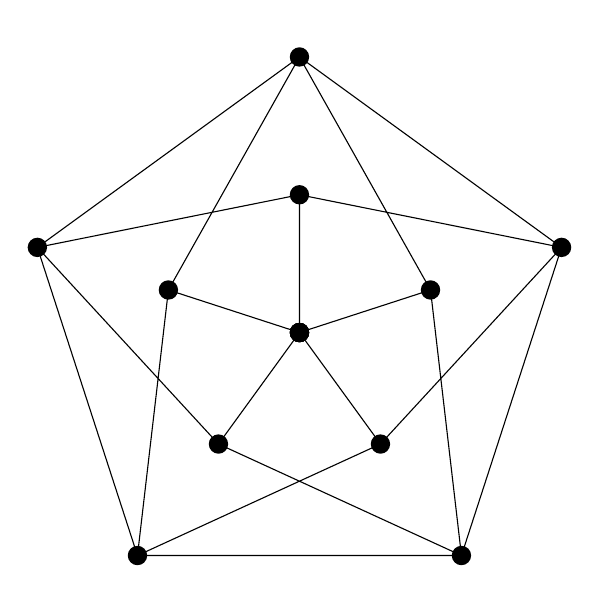
\begin{tikzpicture}[scale=1.75]
        \foreach \x in {0,...,4}{
            \draw (0,0) \v -- (90+\x*72:1) \v -- (162+\x*72:2) \v -- (90+\x*72:2) -- (162+\x*72:1);
        }
    \end{tikzpicture}
    \item Based on the drawing of the graph $G$ above, can you conclude whether or not $G$ is planar? Why or why not?
\end{enumerate}

%%%%%%%%%%%%%%%%%%%%%%%%%%%%%%%%%%%%%%%%%%%%%%%%%%%%%%%%%
\pagebreak
%%%%%%%%%%%%%%%%%%%%%%%%%%%%%%%%%%%%%%%%%%%%%%%%%%%%%%%%%
\section{Learning target G3, version 1}
\begin{enumerate}
    \item Find the chromatic number of the graph below, and show me a proper coloring.
    \begin{center}
        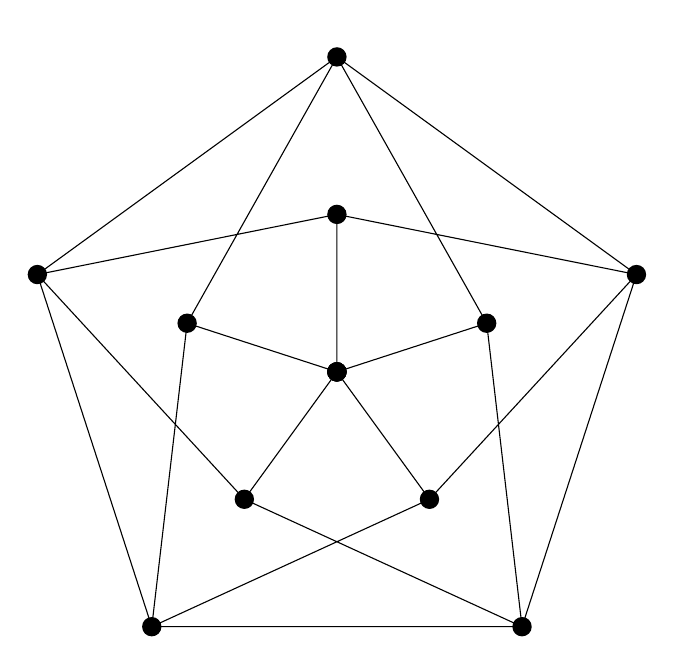
\begin{tikzpicture}[scale=2]
            \foreach \x in {0,...,4}{
                \draw (0,0) \v -- (90+\x*72:1) \v -- (162+\x*72:2) \v -- (90+\x*72:2) -- (162+\x*72:1);
            }
        \end{tikzpicture}
    \end{center}
    \item Prove that you're right. (That is, give a convincing reason why the chromatic number isn't \textit{less} than the number of colors you used.)
\end{enumerate}

%%%%%%%%%%%%%%%%%%%%%%%%%%%%%%%%%%%%%%%%%%%%%%%%%%%%%%%%%
\pagebreak
%%%%%%%%%%%%%%%%%%%%%%%%%%%%%%%%%%%%%%%%%%%%%%%%%%%%%%%%%
\section{Learning target P2, version 2}
This is true: If $G'$ is a subgraph of a bipartite graph $G$, then $G'$ is bipartite.
\begin{enumerate}[leftmargin=0pt]
    \item Write a framework for a direct proof.
    \vfill
    \item Write a framework for a proof by contrapositive.
    \vfill
    \item Write a framework for a proof by contradiction.
    \vfill
\end{enumerate}

%%%%%%%%%%%%%%%%%%%%%%%%%%%%%%%%%%%%%%%%%%%%%%%%%%%%%%%%%
\pagebreak
%%%%%%%%%%%%%%%%%%%%%%%%%%%%%%%%%%%%%%%%%%%%%%%%%%%%%%%%%
\section{Learning target P1, version 2}
Prove that if $G'$ is a subgraph of a bipartite graph $G$, then $G'$ is bipartite.

Use one of your frameworks from the P2 problem.

%%%%%%%%%%%%%%%%%%%%%%%%%%%%%%%%%%%%%%%%%%%%%%%%%%%%%%%%%
\pagebreak
%%%%%%%%%%%%%%%%%%%%%%%%%%%%%%%%%%%%%%%%%%%%%%%%%%%%%%%%%
\section{Learning target L1 / L2 / L3, version 2}
Consider the following statement: Every tree is planar.
\begin{enumerate}
    \item[\textbf{L1}.] Translate this into ``if-then'' form in human language:

    \vspace{2cm}
    and then translate your human ``if-then'' version into properly quantified symbols.

    \vspace{2cm}
    \item[\textbf{L2}.] Write the contrapositive, converse, and inverse of this statement in human words.

    Contrapositive:

    \vspace{2cm}
    Inverse:

    \vspace{2cm}
    Converse:

    \vspace{2cm}
    \item[\textbf{L3}.] Write the negation of the original statement in symbols, and translate it into human words.
    
    \vfill
    \item[\textbf{Bonus}:] Prove or disprove this statement. Use the back of this page.
\end{enumerate}

%%%%%%%%%%%%%%%%%%%%%%%%%%%%%%%%%%%%%%%%%%%%%%%%%%%%%%%%%
\pagebreak
%%%%%%%%%%%%%%%%%%%%%%%%%%%%%%%%%%%%%%%%%%%%%%%%%%%%%%%%%
\section{Learning target L4, version 2}
Are the two compound logical statements below logically equivalent or not? Include a truth table and a clear explanation.
\[
(P \land Q) \rightarrow R \hspace{40pt} \lnot P \lor \lnot Q \lor R
\]


\iffalse
<Graph indexType="custom" height="400" width="400" nodes={[{label:"dog",center:{x:141.2,y:180.2}},{label:"cat",center:{x:274.8,y:335.8}},{label:"cow",center:{x:206,y:332.9}},{label:"bear",center:{x:257.2,y:140}},{label:"fish",center:{x:332.2,y:233.6}},{label:"bird",center:{x:143.4,y:283.5}}]} edges={[{source:1,target:3},{source:0,target:3},{source:3,target:4},{source:1,target:4},{source:0,target:4},{source:0,target:5},{source:5,target:2},{source:5,target:3},{source:5,target:4}]} />
\fi

\iffalse
<Graph indexType="custom" height="400" width="400" nodes={[{label:"A",center:{x:178.2,y:78.3}},{label:"B",center:{x:166.2,y:185}},{label:"C",center:{x:296.2,y:225.6}},{label:"D",center:{x:218.1,y:172.2}},{label:"E",center:{x:104.9,y:270.2}},{label:"F",center:{x:198,y:209.7}}]} edges={[{source:0,target:2},{source:2,target:3},{source:0,target:4},{source:1,target:4},{source:2,target:4},{source:0,target:5},{source:1,target:5},{source:4,target:5},{source:2,target:5}]} />
\fi

\end{document}